% Document Type Management
    \documentclass{book}
    \usepackage[utf8]{inputenc}
    \usepackage[english]{babel}
     
 
%  Packages for Bibiography Management
%    \usepackage{biblatex}
%    \usepackage{csquotes}
%    \addbibresource{references.bib}

% AMS Packages
    \usepackage{amsfonts}
    \usepackage{amssymb}
    \usepackage{amsmath}
    \usepackage{amsthm}
    \usepackage{esvect}
    \usepackage{blindtext}


% Images Management Packages
    \usepackage{tcolorbox}
    \usepackage{graphicx}
    \graphicspath{ {images/} }


% Packages to Draw Images
    \usepackage{float}
    \usepackage{tikz}
    \usetikzlibrary{shapes,backgrounds}
    \usetikzlibrary{positioning}


% Custom Section Labels   
        \newtheorem{theorem}{Theorem}[section]
        \newtheorem{conjecture}[theorem]{Conjecture}
        \newtheorem{corollary}{Corollary}[theorem]
        \newtheorem{lemma}[theorem]{Lemma}

    \theoremstyle{definition}
        \newtheorem{definition}{Definition}[section]
        \newtheorem{example}{Example}[definition]
        \newtheorem{entry}{Entry}[definition]
 
    \theoremstyle{remark}
        \newtheorem{remark}{Remark}





% Custom Chapters and Sections
    \usepackage{titlesec}
    
    \renewcommand\contentsname{Table of Contents}
    \titleformat{\chapter}[display]
      {\bfseries\large}
      {\filleft\MakeUppercase{\chaptertitlename} \large\thechapter}
      {2ex}
      {\titlerule\vspace{2ex}\filleft}
    \titleformat{name=\chapter,numberless}[display]
      {\bfseries\large}
      {\titlerule}
      {-7ex}
      {\filleft\MakeUppercase}[\vspace{5ex}]
    \titlespacing*{\chapter}{0pt}{120pt}{6pt}


% Custom Commands '
    \newcommand{\bb}[1]{\mathbb{#1}}
    \newcommand{\cc}[1]{\mathcal{#1}}
    \newcommand{\ovec}{\big \langle}
    \newcommand{\cvec}{\big \rangle}
    \newcommand{\m}{\cdot}



\begin{document}

\begin{comment}

\tikz 
    \draw (100pt,100pt) --(20pt, 6pt);
    
\tikz
    \fill[orange] (2ex,2ex) 
    circle (2ex);

\tikz
    \draw (0,0) -- (1,0) -- (1,1) -- cycle;

\newpage    
\tikz
    \draw [thick,rounded, corners=8p]
    (0,0) -- (0,2) -- (1,3.25) -- (2,2) -- (2,0) -- (0,2) -- (2,2) -- (0,0) -- (2,0);

\end{comment}




\begin{tikzpicture}
    \draw (-1.5,0) -- (1.5,0);
    \draw (0,-1.5) -- (0, 1.5);
\end{tikzpicture}

\begin{comment}
Failed to compile locally and in the cloud
    \begin{tikzpicture}
        \filldraw [gray]    (0,0) circle [radius=2pt]
                            (1,1) circle [radius=2pt]
                            (2,1) circle [radius=2pt]
                            (2,0) circle [radius=2pt]
        \draw (0,0) .. controls (1,1) and (2,1) ... (2,0);
    \end{tikzpicture}




    \begin{tikzpicture}
        \filldraw [gray]    (0,0) circle [radius=2pt]
                            (1,1) circle [radius=2pt]
                            (2,1) circle [radius=2pt]
                            (2,0) circle [radius=2pt]
        \draw (0,0) .. controls (1,1) and (2,1) .. (2,0);
    \end{tikzpicture}
\end{comment}   

Next well draw a half circle \\
\begin{tikzpicture}
    \draw (-1.5,0) -- (1.5,0);
    \draw (0,-1.5) -- (0, 1.5);
    \draw (-1, 0) ..    controls (-1, 0.555) and (-0.555,1) .. (0,1)
                  ..    controls (0.555, 1) and (1, 0.555) .. (1,0);
    \end{tikzpicture}

Next we will use simplier commands to draw circular figures \\
    \tikz 
        \draw (0,0) circle [radius=10pt];
        
    \tikz
        \draw (0,0) ellipse [x radius=20pt, y radius=10pt];
        
Next, we will draw a full circle on the xy plain \\
    \begin{tikzpicture}
        \draw (-1.5,0) -- (1.5,0);
        \draw (0,-1.5) -- (0,1.5);
        \draw (0,0) circle [radius=1cm];
    \end{tikzpicture}

\newpage
Custom Mathematical Engine Example \\

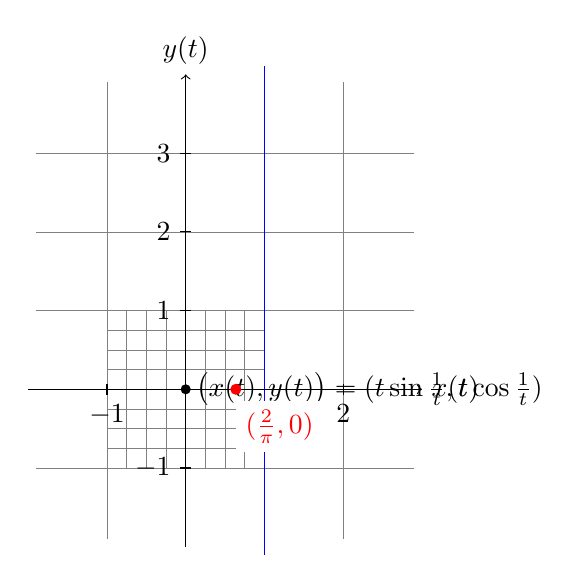
\begin{tikzpicture}
    \draw[gray,very thin] (-1.9,-1.9) grid (2.9,3.9)
    [step=0.25cm] (-1,-1) grid (1,1);
    \draw[blue] (1,-2.1) -- (1,4.1); % asymptote
    \draw[->] (-2,0) -- (3,0) node[right] {$x(t)$};
    \draw[->] (0,-2) -- (0,4) node[above] {$y(t)$};
    \foreach \pos in {-1,2}
    \draw[shift={(\pos,0)}] (0pt,2pt) -- (0pt,-2pt) node[below] {$\pos$};
    \foreach \pos in {-1,1,2,3}
    \draw[shift={(0,\pos)}] (2pt,0pt) -- (-2pt,0pt) node[left] {$\pos$};
    \fill (0,0) circle (0.064cm);
    \draw[thick,parametric,domain=0.4:1.5,samples=200]
    % The plot is reparameterised such that there are more samples
    % near the center.
    plot[id=asymptotic-example] function{(t*t*t)*sin(1/(t*t*t)),(t*t*t)*cos(1/(t*t*t))}
    node[right] {$\bigl(x(t),y(t)\bigr) = (t\sin \frac{1}{t}, t\cos \frac{1}{t})$};
    \fill[red] (0.63662,0) circle (2pt)
    node [below right,fill=white,yshift=-4pt] {$(\frac{2}{\pi},0)$};
\end{tikzpicture}





\end{document}